\section{Coupled Results}
\label{sec:coupledResults}

\begin{frame}{Remember why we are here}
  \pause
  \huge Model a nuclear reactor.
\end{frame}

\begin{frame}{\gls{abr} -- MET-1000}
  \begin{itemize}
    \item Benchmark published February 2016 \cite{abr}.
    \item Four designs including MET-1000.
    \item Thirty-one solutions including \dif.
  \end{itemize}
  \vspace{0.2in}
  \begin{itemize}
    \item Eighteen cross-section regions.
    \item Forty-Nine material compositions.
    \item Dimensions and isotopic compositions fully specified.
    \item Cross sections generated independently.
  \end{itemize}
\end{frame}

\begin{frame}{Benchmark Result}
  \vspace{-0.25in}
  \begin{figure}
    \centering
    \subfloat[$\phi_{1}$]{
      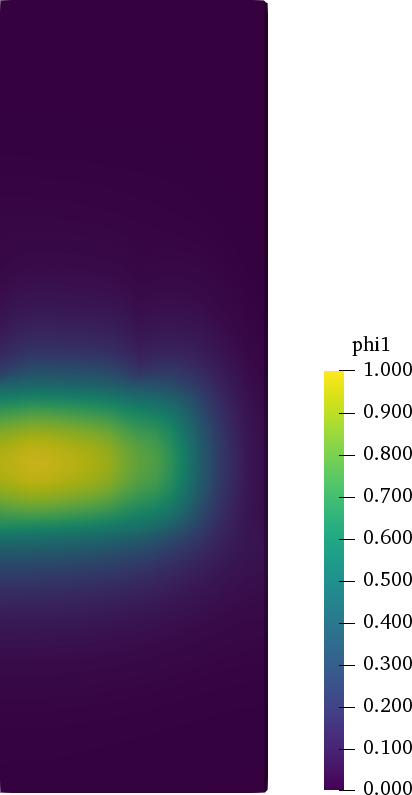
\includegraphics[width=0.30\textwidth]{abr_phi_nod_group1}}
    \hspace{1in}
    \subfloat[$\phi_{2}$]{
      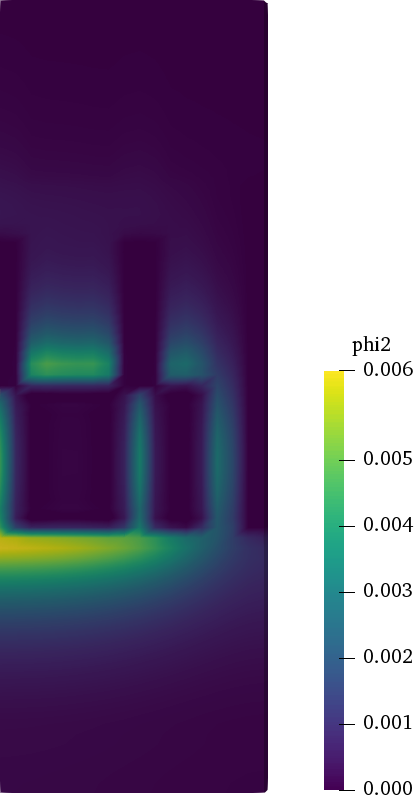
\includegraphics[width=0.30\textwidth]{abr_phi_nod_group2}}
  \end{figure}
  \begin{block}{}
    \centering
    $\keff =  1.006694 $ \qquad (\dif $-700\units{\glsentryshort{pcm}}$)
  \end{block}
\end{frame}

\begin{frame}{Reactivity Coefficients}
  The reactivity of a reactor can be defined.
  \begin{equation}
    \label{eq:reactivity}
    \rho_i = \frac{\keffsub{i} - 1}{\keffsub{i}}
  \end{equation}
  A general reactivity coefficient is a derivative with respect to a variable of
  interest.
  \begin{align}
    \label{eq:reactivity_coefficient}
    \alpha_x(x_i) &= \left. \frac{\partial \rho}{\partial x} \right|_{x=x_i} \\
    \Delta \rho &\approx \alpha_x(x_i) \, \Delta x
  \end{align}
\end{frame}

\begin{frame}
  Consider a series of reactor powers $Q_{Rx,i} = \{0\%,\ldots,100\%\}$.
  Define the following reactivity coefficients.
  \begin{align}
    \label{eq:power_reactivity_coefficient}
    \alpha_{power}(Q_{Rx,i}) &= \frac{\rho(Q_{Rx,i}) - \rho(Q_{Rx,i} + 
      \Delta Q_{Rx})} {\Delta Q_{Rx}} \\
    \label{eq:thermal_expansion_reactivity_coefficient}
    \alpha_{thexp}(Q_{Rx,i}) &= \frac{\rho(\texp(Q_{Rx,i})) -
      \rho(\texp(Q_{Rx,i} + \Delta Q_{Rx}))}{\Delta Q_{Rx}} \\
    % (coolant temperature coefficient)
    \label{eq:doppler_reactivity_coefficient}
    \alpha_{CTC}(Q_{Rx,i}) &= \frac{\rho(Q_{Rx,i}) - \rho(T_{cool} + 
      \Delta T_{cool})} {\Delta T_{cool}} \\
    \label{eq:coolant_temperature_reactivity_coefficient}
    \alpha_{Doppler}(Q_{Rx,i}) &= \frac{\rho(Q_{Rx,i}) - \rho_i(T_{fuel} + 
      \Delta T_{fuel})} {\Delta T_{fuel}}
  \end{align}
\end{frame}

\begin{frame}{Eigenvalue Feedback}
  \begin{figure}
    \centering
    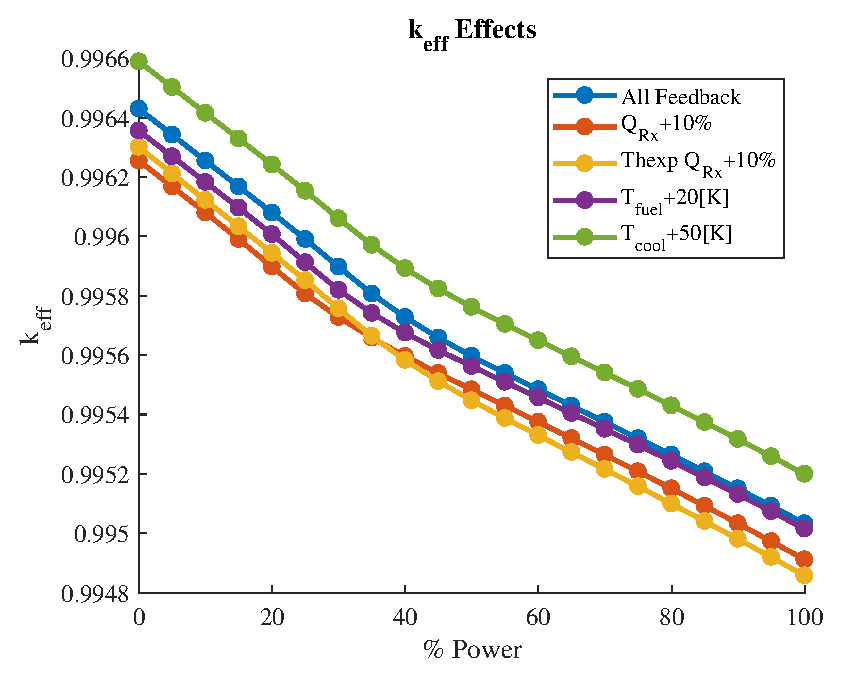
\includegraphics[width=0.7\textwidth]{keff_effects}
    \caption{\keff Feedback Effects.}
    \label{fig:keff_effects}
  \end{figure}
\end{frame}

\begin{frame}{Temperature Reactivity Coefficients}
  \begin{figure}
    \centering
    \subfloat{
      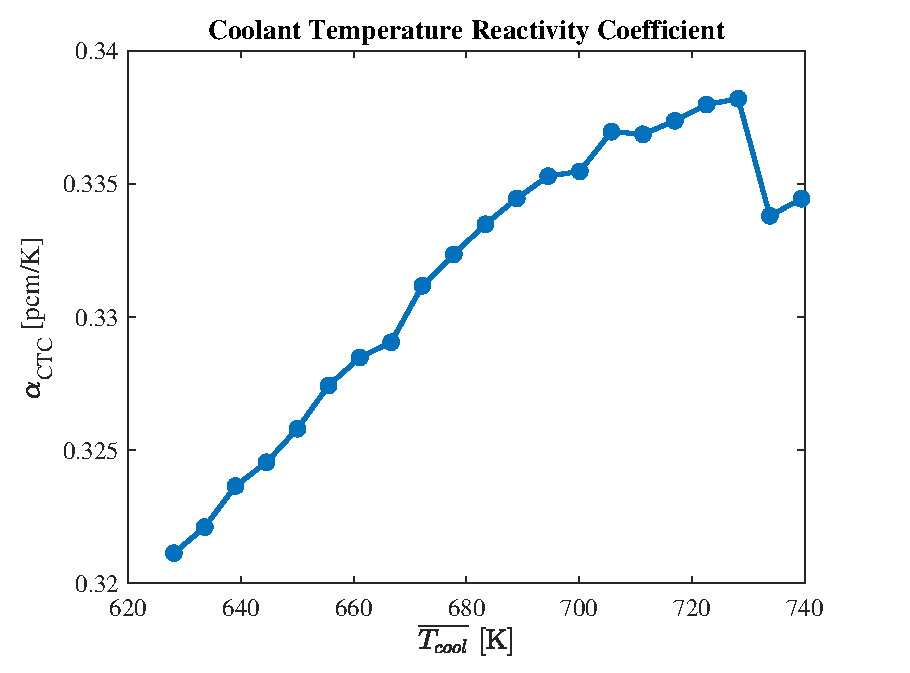
\includegraphics[width=0.5\textwidth]{alpha_cool}}
    \hspace*{\fill}
    \subfloat{
      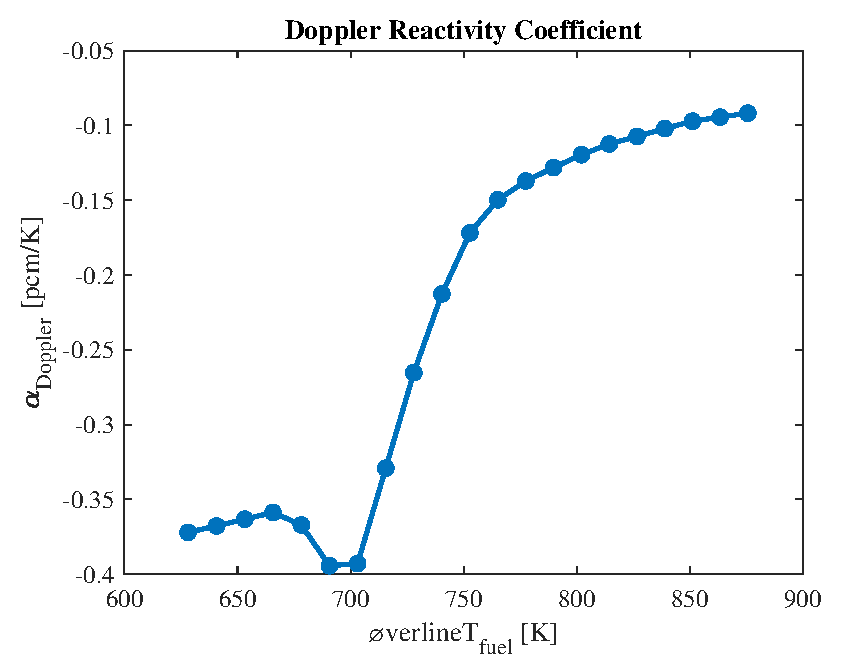
\includegraphics[width=0.5\textwidth]{alpha_fuel}}
  \end{figure}
\end{frame}

\begin{frame}{Power Reactivity Coefficients}
  \begin{figure}
    \centering
    \subfloat{
      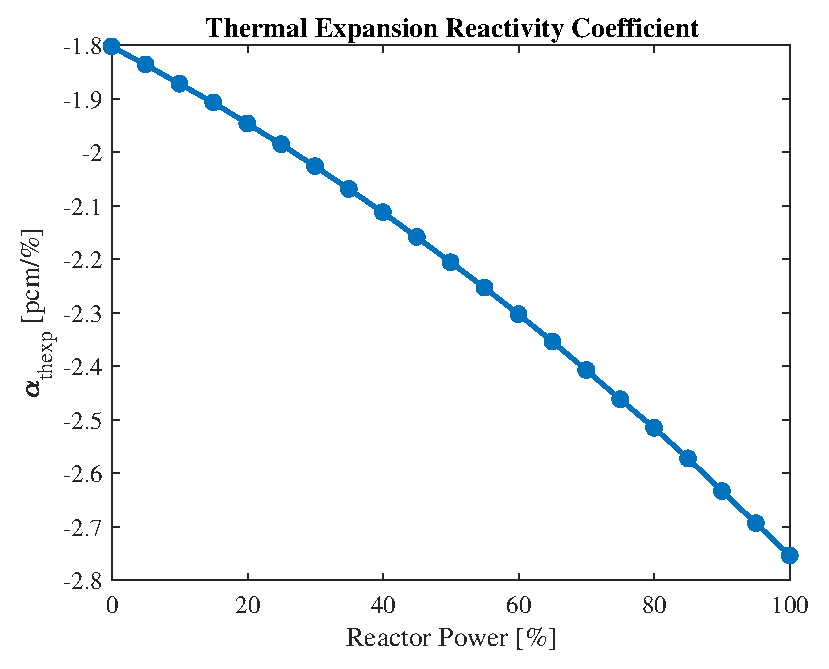
\includegraphics[width=0.5\textwidth]{alpha_thexp}}
    \hspace*{\fill}
    \subfloat{
      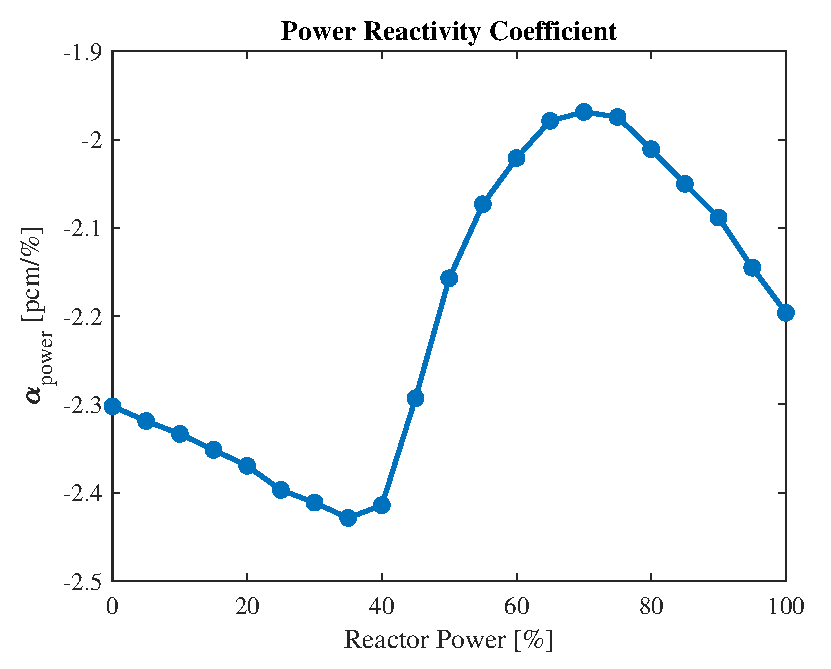
\includegraphics[width=0.5\textwidth]{alpha_power}}
  \end{figure}
\end{frame}
